\documentclass[11pt]{beamer}
\usetheme{Madrid}
\usepackage[utf8]{inputenc}
\usepackage{url}


\title{Introduction to Computational Science}
\subtitle{Optimizing Traffic Lights in Urban Street Grids}
\author{Klaas Kliffen, Jan Kramer}
\setbeamertemplate{navigation symbols}{}
\date{January 7, 2016}

\begin{document}
\maketitle

% the problem:
\begin{frame}{Introduction}
% What did we model
\begin{figure}
\centering
\includegraphics[width=.45\textwidth]{trafficlighttree.jpg}
\end{figure}
\end{frame}

\begin{frame}{The problem}
\begin{itemize}
    \item analyze different traffic light solutions
    \item "American city" grid
    \item uniform traffic
\end{itemize}
\end{frame}

% the solution method:
\begin{frame}{Method overview}
% Global overview of the simulatar
\begin{itemize}
    \item 9 intersection
    \item wrapped boundaries
    \item different traffic light heuristics
    \item gather data
\end{itemize}
\end{frame}

% the implementation:
\begin{frame}{Intersection design}

\begin{itemize}
 \item intersections define the grid
 \item 8 lanes per intersection which resemble fixed length queues
 \begin{itemize}
  \item 2 per direction:
  \item 1 for turning left
  \item 1 for forward and turning right
 \end{itemize}
 \item traffic light controls lanes
 \item On queuing of a car, chooses randomly one of two lanes of the next intersection (if available)


\end{itemize}
\end{frame}

\begin{frame}{Statistics gathering}
% What did we collect?
\begin{itemize}
\item average waiting time
\item average throughput
\item future: minima and maxima
\end{itemize}
\end{frame}

\begin{frame}{Demo}
\begin{figure}
\centering
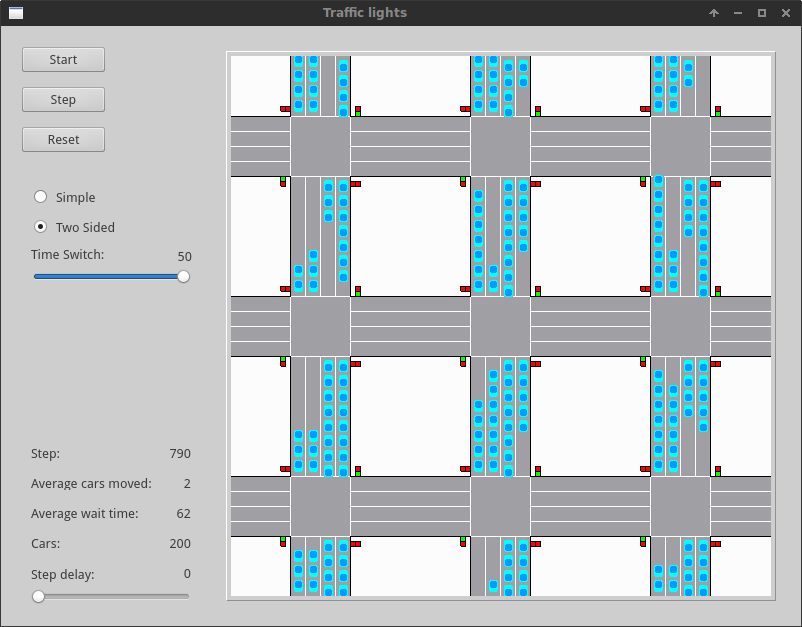
\includegraphics[width=.8\textwidth]{vertical.png}
\end{figure}
\end{frame}


\begin{frame}{Results: pattern}
%What did we find
\begin{itemize}
 \item A pattern emerged with long switch timings on the two sided algorithm
 \item It would alternate between two states with 1 switch step of chaos
\end{itemize}
\begin{columns}
    \begin{column}{.5\textwidth}
        \begin{figure}
        \centering
        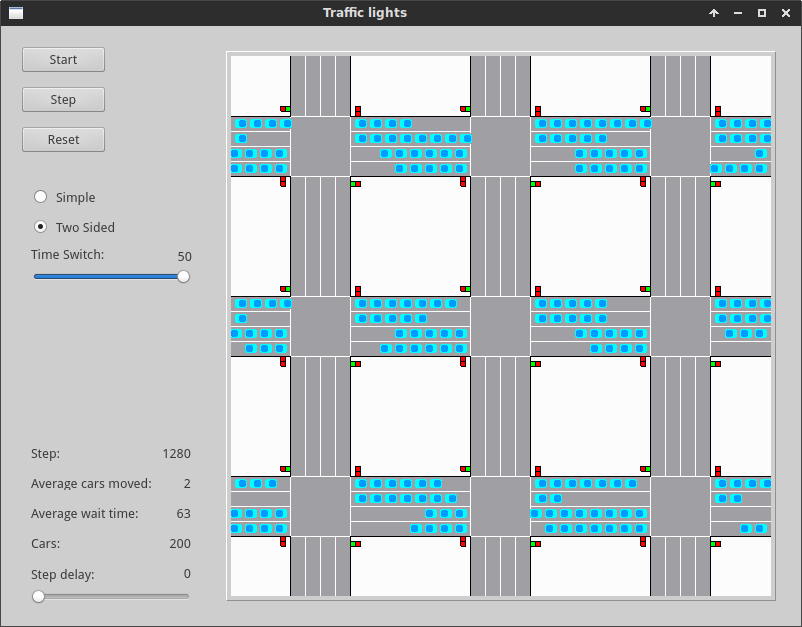
\includegraphics[width=\textwidth]{horizontal.png}
        \end{figure}
    \end{column}
    \begin{column}{.5\textwidth}
        \begin{figure}
        \centering
        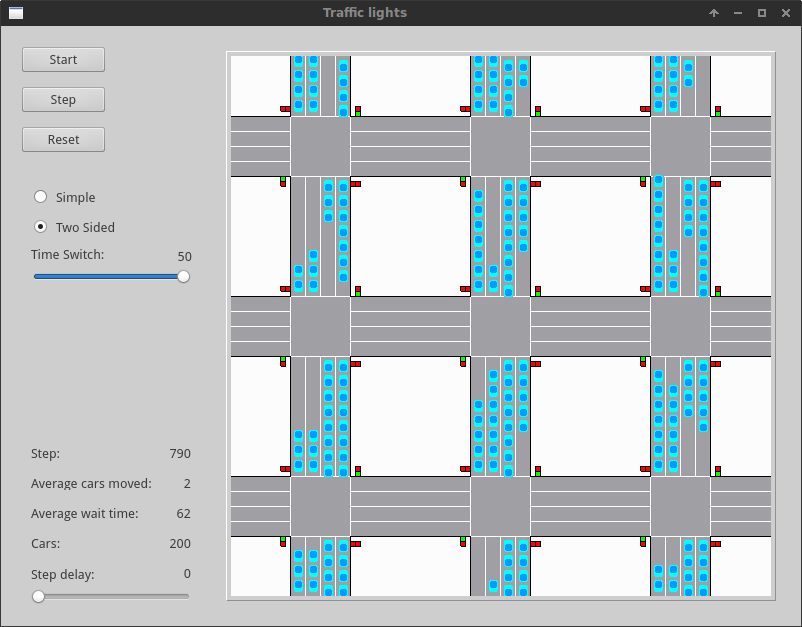
\includegraphics[width=\textwidth]{vertical.png}
        \end{figure}
    \end{column}
\end{columns}

\end{frame}


\begin{frame}{Results: mean car waiting time}
\textbf{Definition:} cars that cannot move to the next field, either to a 
red traffic light or another car. Averaged over all lanes.\\~\\
Measured using 200 cars simulating 5000 steps.

\begin{table}
\centering
\begin{tabular}{l|c|c|c|c|c}
algorithm/switch time & 1 & 4 & 8 & 16 & 32\\
\hline
simple & 6 & 8 & 13 & 23 & 48\\
two sided & 6 & 7 & 8 & 18 & 39\\
\end{tabular}
\end{table}
 
\end{frame}

\begin{frame}{Results: cars moved per 9 intersections per step}
\textbf{Definition:} total car count that passed a traffic light during a step.
Averaged over all steps.\\~\\
Measured using 200 cars simulating 5000 steps.
\begin{table}
\centering
\begin{tabular}{l|c|c|c|c|c}
algorithm/switch time & 1 & 4 & 8 & 16 & 32\\
\hline
simple & 14 & 12 & 9 & 6 & 3\\
two sided & 13 & 12 & 12 & 7 & 4\\
\end{tabular}
\end{table}
 
\end{frame}


\begin{frame}{Conclusion}

\begin{itemize}
 \item 
\end{itemize}

    
\end{frame}

\begin{frame}{Introduction to Computational Science}
\begin{center}
{\large Optimizing Traffic Lights in Urban Street Grids}\\
\end{center}

\begin{center}
Klaas Kliffen, Jan Kramer
\end{center}

%TODO: put a nice image here (instead of asking for questions)
    
\end{frame}



\end{document}
